% ════════════════════════════════════════════════════════════════
\subsection{Termin 1}
% ════════════════════════════════════════════════════════════════

\begin{zadanie}[Zadanie 1 --- wszystkie liście Huffmana na tej samej głębokości (15 p.)]
	Niech $T$ będzie optymalnym drzewem Huffmana dla $|A|=2^k$ symboli, przy czym
	dla każdych trzech symboli $f(x)+f(y)>f(z)$. Udowodnij, że wszystkie liście
	$T$ mają głębokość~$k$.
\end{zadanie}

Warunek ,,$f(x)+f(y)>f(z)$ dla wszystkich trójek'' oznacza, że \uemph{suma
dwóch najmniejszych częstości przewyższa największą}. Pokażemy indukcyjnie po~$k$,
że algorytm Huffmana buduje pełne drzewo binarne głębokości~$k$.

\paragraph{Krok bazowy.}
Dla $k=0$ mamy jeden symbol, drzewo to pojedynczy liść na głębokości~$0$.

\paragraph{Krok indukcyjny.}
Niech $n=2^k$ i~$f_1\le f_2\le\dots\le f_n$. Załóżmy $f_1+f_2>f_n$.

\emph{Najpierw kojarzone są same liście.} Algorytm łączy dwie najmniejsze
częstości w~węzeł $w=f_1+f_2$. Z~założenia $w=f_1+f_2>f_n\ge f_i$ dla każdego
oryginalnego liścia, więc każdy nowo utworzony węzeł wewnętrzny ma wagę większą
niż dowolny pozostały liść. W~konsekwencji, dopóki istnieją niepołączone
oryginalne liście, dwie najmniejsze wagi w~kolejce są zawsze liśćmi --- algorytm
najpierw paruje wszystkie $2^k$ liści w~$2^{k-1}$ węzłów, tworząc kompletny
najniższy poziom.

\emph{Nowe wagi spełniają ten sam warunek.} Po~sparowaniu mamy $2^{k-1}$ wag
$w_1,\dots,w_{2^{k-1}}$, każda będąca sumą pewnej pary liści, więc
$w_i\ge f_1+f_2>f_n$. Każda waga to suma dwóch liści, więc największa
$\le f_{n-1}+f_n$. Stąd suma dwóch najmniejszych nowych wag spełnia
\[
	w_i+w_j\ >\ 2f_n\ \ge\ f_{n-1}+f_n\ \ge\ \max_\ell w_\ell,
\]
czyli warunek ,,suma dwóch najmniejszych $>$ największa'' zachodzi dla nowej
rodziny $2^{k-1}$ wag.

Z~założenia indukcyjnego algorytm zbuduje na tych wagach pełne drzewo
głębokości $k-1$; doczepienie pod każdym jego liściem pary liści oryginalnych
daje pełne drzewo głębokości~$k$. Wszystkie liście $T$ leżą więc na
głębokości~$k$. $\qed$

\clearpage
\begin{zadanie}[Zadanie 2 --- najtańszy element w~bazie minimalnej (15 p.)]
	Matroid $M=(S,\mathcal{I})$, wagi $w:S\to\mathbb{R}_+$, $S\ni x$ minimalizuje
	$w(x)$. Udowodnij, że $x$ należy do pewnej bazy o~minimalnej wadze 
(innymi słowy: istnieje zbiór $I \in \mathcal{I}$ taki, że $x\in I$ oraz $w(i) = \min_{J\in\mathcal{I}}w(J)$.
\end{zadanie}

Zauważmy, że $x$ nie jest pętlą, tzn. $\{x\}\in\mathcal{I}$. Gdyby bowiem $\{x\}$
było zależne, to $\{x\}$ nie zawierałoby się w~żadnym zbiorze niezależnym, a~więc
$x$ nie należałoby do~żadnej bazy i~teza byłaby fałszywa. Tezę rozumiemy zatem
przy założeniu, że minimalizujący wagę element nie jest pętlą (pętle, jako
nieobecne w~żadnej bazie, można usunąć z~$S$).

\begin{dygresja}
	\emph{Pętlą} w~matroidzie $M=(S,\mathcal{I})$ nazywamy element $x$, dla którego
	już sam jednoelementowy zbiór jest zależny: $\{x\}\notin\mathcal{I}$
	(równoważnie $\operatorname{rank}(\{x\})=0$). Skoro żaden zbiór niezależny nie
	może zawierać pętli, nie zawiera jej też żadna baza --- pętla nigdy nie wejdzie
	do~rozwiązania, więc spokojnie pomijamy ją w~rozważaniach. Nazwa pochodzi
	od~matroidu grafowego: krawędź będąca pętlą (łączącą wierzchołek z~samym sobą)
	sama tworzy cykl, więc nie należy do~żadnego lasu.

	W~matroidzie liniowym (gdzie $S$ to zbiór wektorów, a~niezależność to liniowa
	niezależność) pętlą jest wektor zerowy: $\{\mathbf{0}\}$ jest zależny, bo
	$1\cdot\mathbf{0}=\mathbf{0}$, więc $\mathbf{0}$ nie wchodzi do~żadnej bazy.
\end{dygresja}

\paragraph{Rozwiązanie (algorytm zachłanny).}
Algorytm zachłanny dla matroidów (Rado--Edmonds,
Twierdzenie~\ref*{N-thm:rado-edmonds}) sortuje elementy rosnąco po~wadze i~kolejno
dokłada do~budowanego zbioru każdy element, który zachowuje niezależność;
zwracany zbiór jest bazą o~minimalnej wadze. Element $x$ ma najmniejszą wagę, więc
przy odpowiednim porządku jest rozważany jako pierwszy, a~ponieważ $\{x\}\in\mathcal{I}$,
zostaje dodany do~budowanej bazy. Zatem zwrócona baza ma minimalną wagę i~zawiera
$x$, co dowodzi tezy. $\qed$

\medskip
\noindent\emph{Alternatywnie (dla ciekawych) --- argument wymiany przez obwody.}
Poniższy dowód nie odwołuje się do~poprawności algorytmu zachłannego, lecz wprost
przekształca dowolną bazę minimalną tak, by zawierała~$x$. Wymaga jednak pojęcia
obwodu, którego nie wprowadzaliśmy na~wykładzie.

\paragraph{Obwody.}
\emph{Obwodem} (cyklem) matroidu nazywamy minimalny zbiór zależny: $\mathcal{C}$
jest obwodem, gdy $\mathcal{C}\notin\mathcal{I}$, ale każdy jego właściwy podzbiór
jest niezależny. W~matroidzie grafowym są to dokładnie zwykłe cykle grafu, stąd
nazwa.

\begin{dygresja}
	Skorzystamy z~\emph{aksjomatu eliminacji obwodów}: jeśli
	$\mathcal{C}_1\ne\mathcal{C}_2$ są obwodami i~$e\in\mathcal{C}_1\cap\mathcal{C}_2$,
	to istnieje obwód $\mathcal{C}_3\subseteq(\mathcal{C}_1\cup\mathcal{C}_2)
	\setminus\{e\}$. W~matroidzie grafowym: dwa cykle dzielące krawędź $e$ sklejone
	wzdłuż~$e$ i~pozbawione $e$ wciąż zawierają jakiś cykl. Aksjomat ten (wraz z~tym,
	że $\emptyset$ nie jest obwodem i~żaden obwód nie zawiera się w~innym) jest
	równoważną charakteryzacją matroidu przez rodzinę obwodów.
\end{dygresja}

Wykorzystamy dwie własności:
\begin{itemize}
	\item jeśli $I\in\mathcal{I}$, a~$I\cup\{x\}\notin\mathcal{I}$, to $I\cup\{x\}$
		zawiera \emph{dokładnie jeden} obwód, i~przechodzi on przez~$x$. \emph{Istnienie:}
		każdy zbiór zależny zawiera obwód (jego minimalny zależny podzbiór), a~ten
		musi zawierać $x$ --- inaczej leżałby w~niezależnym $I$. \emph{Jedyność:}
		gdyby były dwa różne obwody $\mathcal{C}_1,\mathcal{C}_2\subseteq I\cup\{x\}$,
		oba zawierałyby $x$, więc z~aksjomatu eliminacji obwodów (dla
		$x\in\mathcal{C}_1\cap\mathcal{C}_2$ istnieje obwód
		$\mathcal{C}_3\subseteq(\mathcal{C}_1\cup\mathcal{C}_2)\setminus\{x\}$)
		dostalibyśmy obwód zawarty w~$I$ --- sprzeczność z~$I\in\mathcal{I}$;
	\item (wymiana) jeśli $\mathcal{C}$ jest obwodem i~$y\in\mathcal{C}$, to
		usunięcie $y$ z~tego zbioru zależnego przywraca niezależność --- to wprost
		definicja: $\mathcal{C}\setminus\{y\}$ jest właściwym podzbiorem obwodu, więc
		jest niezależny.
\end{itemize}

\paragraph{Argument wymiany.}
Niech $B$ będzie dowolną bazą o~minimalnej wadze. Jeśli $x\in B$, gotowe.
W~przeciwnym razie $B\cup\{x\}$ zawiera dokładnie jeden obwód (cykl) $\mathcal{C}$
przechodzący przez~$x$. Obwód ma co najmniej dwa elementy, więc istnieje
$y\in\mathcal{C}\setminus\{x\}\subseteq B$. Z~własności wymiany dla obwodów zbiór
\[
	B'=\big(B\setminus\{y\}\big)\cup\{x\}
\]
jest bazą (usunięcie dowolnego elementu obwodu po~dodaniu $x$ przywraca
niezależność i~zachowuje liczność). Ponieważ $x$ ma najmniejszą wagę,
$w(x)\le w(y)$, więc
\[
	w(B')=w(B)+w(x)-w(y)\le w(B).
\]
Skoro $B$ jest minimalna, $w(B')=w(B)$, czyli $B'$ jest bazą minimalnej wagi
zawierającą~$x$. $\qed$

\clearpage
\begin{zadanie}[Zadanie 3 --- mnożenie macierzy z~32 mnożeniami bloków (15 p.)]
	Dane są wzory mnożące dwie macierze $4\times 4$ za pomocą $32$ mnożeń i~$256$
	dodawań liczb.\footnote{Zakładamy również, że te wzory nie korzystają
	z~przemienności mnożenia.} Skonstruuj rekurencyjny algorytm mnożenia macierzy $n\times n$
	i~wyznacz jego złożoność.
\end{zadanie}

\paragraph{Algorytm.}
Dla $n=4^m$ dzielimy każdą macierz $n\times n$ na siatkę $4\times 4$ bloków
rozmiaru $\tfrac{n}{4}\times\tfrac{n}{4}$. Stosujemy dane wzory traktując bloki
jak ,,skalary'': ponieważ wzory nie korzystają z~przemienności mnożenia, są
poprawne także dla nieprzemiennego mnożenia bloków (macierzy). Wymaga to:
\begin{itemize}[nosep]
	\item $32$ \uemph{mnożeń} bloków $\tfrac n4\times\tfrac n4$ (rekurencyjnie),
	\item $256$ \uemph{dodawań/odejmowań} bloków, każde w~czasie
	      $\BO\!\big((n/4)^2\big)=\BO(n^2)$.
\end{itemize}

\paragraph{Złożoność.}
\begin{flalign*}
	T(n) & = 32\cdot T\!\left(\frac{n}{4}\right) + \BO(n^2) &  & a = 32,\ b = 4,\ k = 2 &  & \\[1.5ex]
	32   & > 4^2 \Rightarrow T(n) = \BT\!\left(n^{\log_4 32}\right) = \BT\!\left(n^{2{,}5}\right) &  &                       &  &
\end{flalign*}
bo $\log_4 32=\tfrac{\log_2 32}{\log_2 4}=\tfrac{5}{2}=2{,}5$. $\qed$

\clearpage
\begin{zadanie}[Zadanie 4 --- minimalny podział grafu na trójkąty (15 p.)]
	Przez \emph{podział grafu $G$ na trójkąty} rozumiemy podział zbioru $V(G)$ na
	trzyelementowe podzbiory $\{u_1,v_1,w_1\},\{u_2,v_2,w_2\},\dots,\{u_k,v_k,w_k\}$,
	gdzie dla każdego $i$ zachodzi $u_iv_i,v_iw_i,u_iw_i\in E(G)$. Jeżeli
	$w\colon E(G)\to\mathbb{R}$, to przez \emph{wagę} takiego podziału rozumiemy sumę
	wag krawędzi wewnątrz klas podziału, tzn. wartość wyrażenia
	$\sum_{i=1}^{k}\big(w(u_iv_i)+w(v_iw_i)+w(u_iw_i)\big)$.

	W~problemie \textsc{Minimum Triangle Partition} mamy dany graf ważony krawędziowo
	i~poszukujemy minimalnej wagi podziału tego grafu na trójkąty. Zaprojektuj
	algorytm, który rozwiąże ten problem w~czasie $\BO^*(2^n)$, gdzie $n$ jest liczbą
	wierzchołków grafu; uzasadnij poprawność i~oszacuj czas działania swojego algorytmu.
\end{zadanie}

\label{sol:triangle-partition}
\paragraph{Programowanie dynamiczne po~podzbiorach.}
Dla $U\subseteq V(G)$ niech $D[U]$ będzie minimalną wagą podziału $U$ na trójkąty
($D[U]=\infty$, gdy $|U|$ nie dzieli się przez $3$ lub podział nie istnieje).
Ustalmy w~$U$ wierzchołek o~najmniejszym indeksie $v=\min U$. W~każdym podziale
$v$ należy do dokładnie jednego trójkąta $\{v,a,b\}$, gdzie $a,b\in U$ oraz
$va,vb,ab\in E(G)$. Stąd
\[
	D[\emptyset]=0,\qquad
	D[U]=\min_{\substack{a,b\in U\setminus\{v\}\\ \{v,a,b\}\text{ --- trójkąt}}}
	\Big(w(va)+w(vb)+w(ab)+D\big[U\setminus\{v,a,b\}\big]\Big).
\]
Odpowiedzią jest $D[V(G)]$.

\begin{alg}{Minimalny podział grafu na trójkąty}{alg:triangle-partition}
	\Function{MinTrianglePartition}{$G,w$}\Comment{zwraca $D[V(G)]$}
	\State $D[\emptyset]\gets 0$
	\For{$U\subseteq V(G)$ rosnąco po~$|U|$, $U\neq\emptyset$}
	\State $D[U]\gets\infty$
	\If{$|U|\bmod 3\neq 0$}\State \textbf{continue}
	\EndIf
	\State $v\gets\min U$
	\For{$a,b\in U\setminus\{v\}$, $a<b$}
	\If{$va,vb,ab\in E(G)$}\Comment{$\{v,a,b\}$ jest trójkątem}
	\State $D[U]\gets\min\big(D[U],\,w(va)+w(vb)+w(ab)+D[U\setminus\{v,a,b\}]\big)$
	\EndIf
	\EndFor
	\EndFor
	\State \Return $D[V(G)]$
	\EndFunction
\end{alg}

\paragraph{Poprawność.}
Ustalenie najmniejszego $v\in U$ usuwa nadmiarowość: każdy podział $U$ ma dokładnie
jeden trójkąt zawierający~$v$ (ten, do którego~$v$ należy), więc rekurencja generuje
każdy podział dokładnie raz --- nie rozpatrujemy tego samego podziału wielokrotnie,
raz „od~trójkąta $\{v,a,b\}$", innym razem od~innej klasy. Reszta $U\setminus\{v,a,b\}$
jest dzielona niezależnie i~optymalnie (optymalna podstruktura). Iterujemy po~wszystkich
możliwych trójkątach zawierających~$v$, więc znajdujemy minimum.

\paragraph{Złożoność.}
Podzbiorów jest $2^n$; dla każdego, przy ustalonym $v$, przeglądamy pary
$(a,b)$ w~czasie $\BO(n^2)$, a~sprawdzenie, czy $\{v,a,b\}$ jest trójkątem
(tzn. $va,vb,ab\in E(G)$), kosztuje $\BO(1)$ przy macierzy sąsiedztwa.
Łącznie $\BO(2^n n^2)=\BO^*(2^n)$ czasu
i~$\BO(2^n)$ pamięci. $\qed$

\clearpage
\begin{zadanie}[Zadanie 5 --- 3-aproksymacyjne kolorowanie grafów dysków jednostkowych (15 p.)]
	Podaj wielomianowy algorytm $3$-aproksymacyjny dla problemu kolorowania grafów
	przecięć dysków jednostkowych\footnote{Przez \emph{graf przecięć dysków
	jednostkowych} rozumiemy tu graf $G$ taki, że $V(G)$ jest skończonym podzbiorem
	$\mathbb{R}^2$ oraz $(x_1,y_1)(x_2,y_2)\in E(G)$ wtedy i~tylko wtedy, gdy
	euklidesowa odległość między punktami $(x_1,y_1)$ i~$(x_2,y_2)$ wynosi nie więcej
	niż~$1$.} i~udowodnij, że współczynnik aproksymacji istotnie wynosi~$3$. Możesz
	pominąć dowód potrzebnego geometrycznego faktu (ale musisz go sformułować).
\end{zadanie}

\label{sol:udg-coloring}
\paragraph{Fakt geometryczny.}
Rozważmy koło o~środku w~$p$ i~promieniu~$1$ (zawiera ono wszystkich sąsiadów
$p$). Jego lewą połowę --- czyli punkty o~współrzędnej $x$ nie większej niż~$x_p$
--- można pokryć trzema wycinkami o~kącie $60^\circ$ każdy. Jeżeli dwa punkty
leżą w~tym samym wycinku i~oba są w~odległości $\le 1$ od~$p$, to są też
w~odległości $\le 1$ od~siebie: cięciwa łuku o~promieniu~$1$ i~kącie $60^\circ$
ma długość $2\sin 30^\circ=1$, a~zatem żadne dwa takie punkty nie są dalej niż
o~tę cięciwę. Wobec tego sąsiedzi $p$ leżący w~jednym wycinku tworzą wraz z~$p$
\uemph{klikę}.

\begin{azfigure}
	\centering
	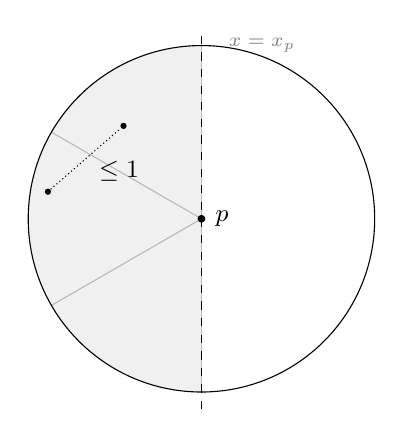
\begin{tikzpicture}[font=\small, >=stealth, scale=2.2]
		% koło o promieniu 1 wokół p; lewa połowa (x <= x_p) pokryta trzema
		% wycinkami po 60 stopni (kąty 90..270 stopni).
		\fill[gray!12] (0,0) -- (90:1) arc (90:270:1) -- cycle;
		\foreach \a in {90,150,210,270} \draw[gray!55] (0,0) -- (\a:1);
		\draw (0,0) circle (1);
		\draw[dashed] (0,-1.1) -- (0,1.1);
		\node[circle, fill, inner sep=1pt, label=right:$p$] at (0,0) {};
		% dwa punkty w jednym wycinku
		\node[circle, fill, inner sep=0.8pt] (a) at (170:0.9) {};
		\node[circle, fill, inner sep=0.8pt] (b) at (130:0.7) {};
		\draw[densely dotted] (a) -- (b);
		\node at (150:0.55) {$\le 1$};
		\node[font=\scriptsize, gray] at (0.35,1.0) {$x=x_p$};
	\end{tikzpicture}
	\caption{Lewa połowa koła o~promieniu~$1$ pokryta trzema wycinkami po~$60^\circ$;
		punkty w~jednym wycinku są wzajemnie w~odległości $\le 1$.}
\end{azfigure}

\paragraph{Algorytm.}
Sortujemy punkty rosnąco po~współrzędnej $x$ i~kolorujemy zachłannie: każdemu
$p$ nadajemy najmniejszy kolor nieużyty przez jego \uemph{wcześniej
pokolorowanych} sąsiadów (czyli tych o~$x\le x_p$).

\paragraph{Współczynnik aproksymacji.}
Wcześniejsi sąsiedzi $p$ leżą w~lewej półpłaszczyźnie koła, więc --- na mocy
faktu --- rozkładają się na $3$ kliki. Każda z~tych klik wraz z~$p$ tworzy klikę,
więc zawiera co najwyżej $\omega-1$ wcześniejszych sąsiadów (gdzie $\omega$ to
liczność największej kliki). Stąd wcześniejszych sąsiadów jest co najwyżej
$3(\omega-1)$, a~algorytm zachłanny nadaje $p$ kolor o~numerze nie większym niż
$3(\omega-1)+1=3\omega-2$. Zatem liczba użytych kolorów spełnia
\[
	\chi_{\text{alg}}\ \le\ 3\omega-2.
\]
Ponieważ każda klika wymaga osobnych kolorów, $\chi\ge\omega$, skąd
\[
	\frac{\chi_{\text{alg}}}{\chi}\ \le\ \frac{3\omega-2}{\omega}\ =\ 3-\frac2\omega\ \le\ 3.
\]
Algorytm jest więc $3$-aproksymacyjny (i~działa w~czasie $\BO(n\log n+m)$). $\qed$
